\documentclass{beamer}
\mode<presentation>

\usepackage{graphicx}

\begin{document}
\title{Stock prices prediction using WT, SAE and LSTM}
\author{Piotr Ambroszczyk, Jan Kociniak}
\date{March 21, 2019}

\begin{frame}
\titlepage
\end{frame}

\begin{frame}
\frametitle{Base paper}
Wei B., Jun Y., Yulei R. (July 2017) \textit{A deep learning framework for financial time series using stacked autoencoders and long-short term memory.}
\end{frame}

\begin{frame}
\frametitle{Flowchart}
\begin{center}
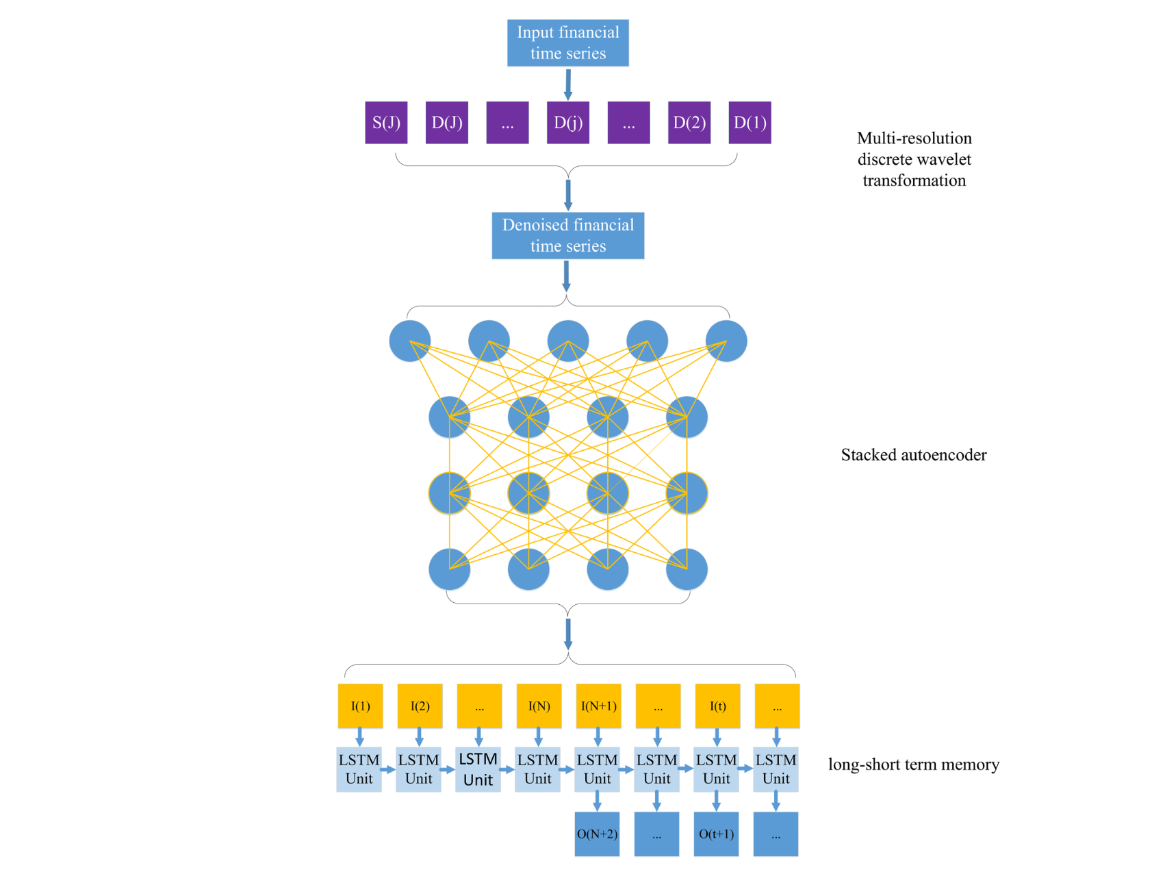
\includegraphics[height=7cm]{flowchart.png}
\end{center}
\end{frame}

\begin{frame}
\frametitle{Denoising}
\begin{minipage}{0.475\textwidth}
\hspace{14pt}Before\vspace{5pt}
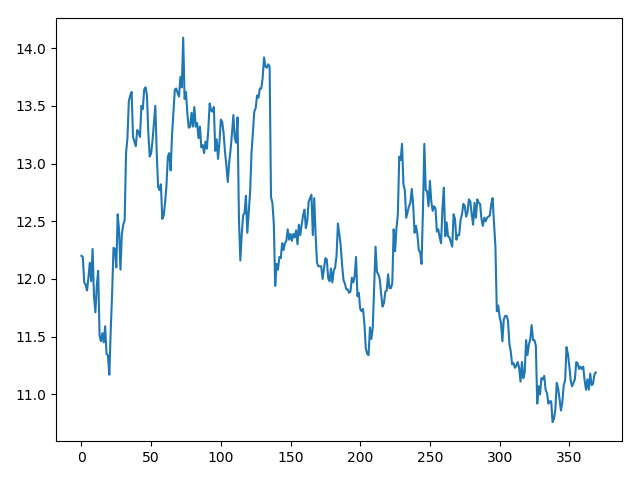
\includegraphics[height=4cm]{before_denoising.png}
\end{minipage}\hspace{10pt}
\begin{minipage}{0.475\textwidth}
\hspace{14pt}After\vspace{5pt}
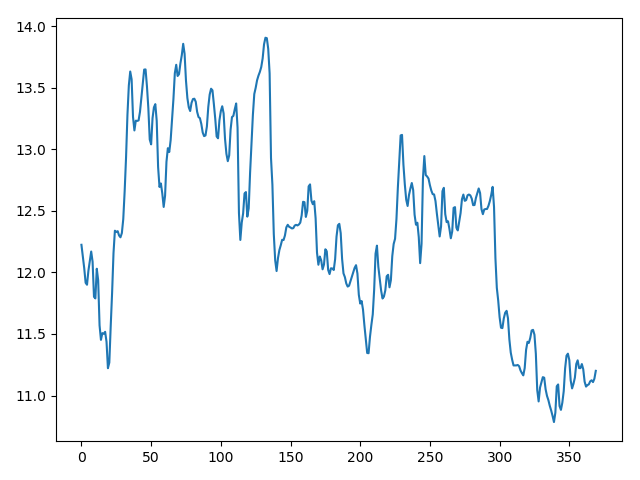
\includegraphics[height=4cm]{after_denoising.png}
\end{minipage}
\end{frame}

\begin{frame}
\frametitle{Wavelet transform}
\begin{center}
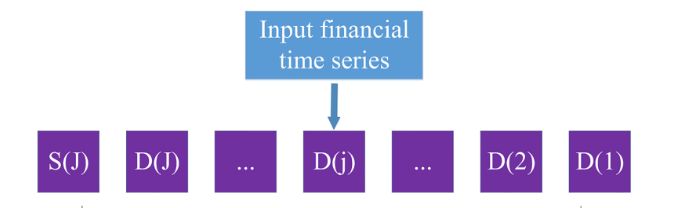
\includegraphics[width=10cm]{wavelet_transform.png}
\end{center}
\end{frame}

\begin{frame}
\frametitle{Wavelet transform}
\begin{itemize}
\item Different decompositions depending on used wavelets.
\item The decomposition is invertible!
\item D1 - the finest coefficients - information about noise.
\item Thresholding = truncating coefficients from Sj, Dj, ..., D1 below given constant.
\item We can compute this constant using D1 coefficients.
\item Apply thresholding and invert!
\end{itemize}
\end{frame}

\begin{frame}
\frametitle{Comparison}
\begin{center}
\begin{tabular}{l r}
Haar wavelet\\
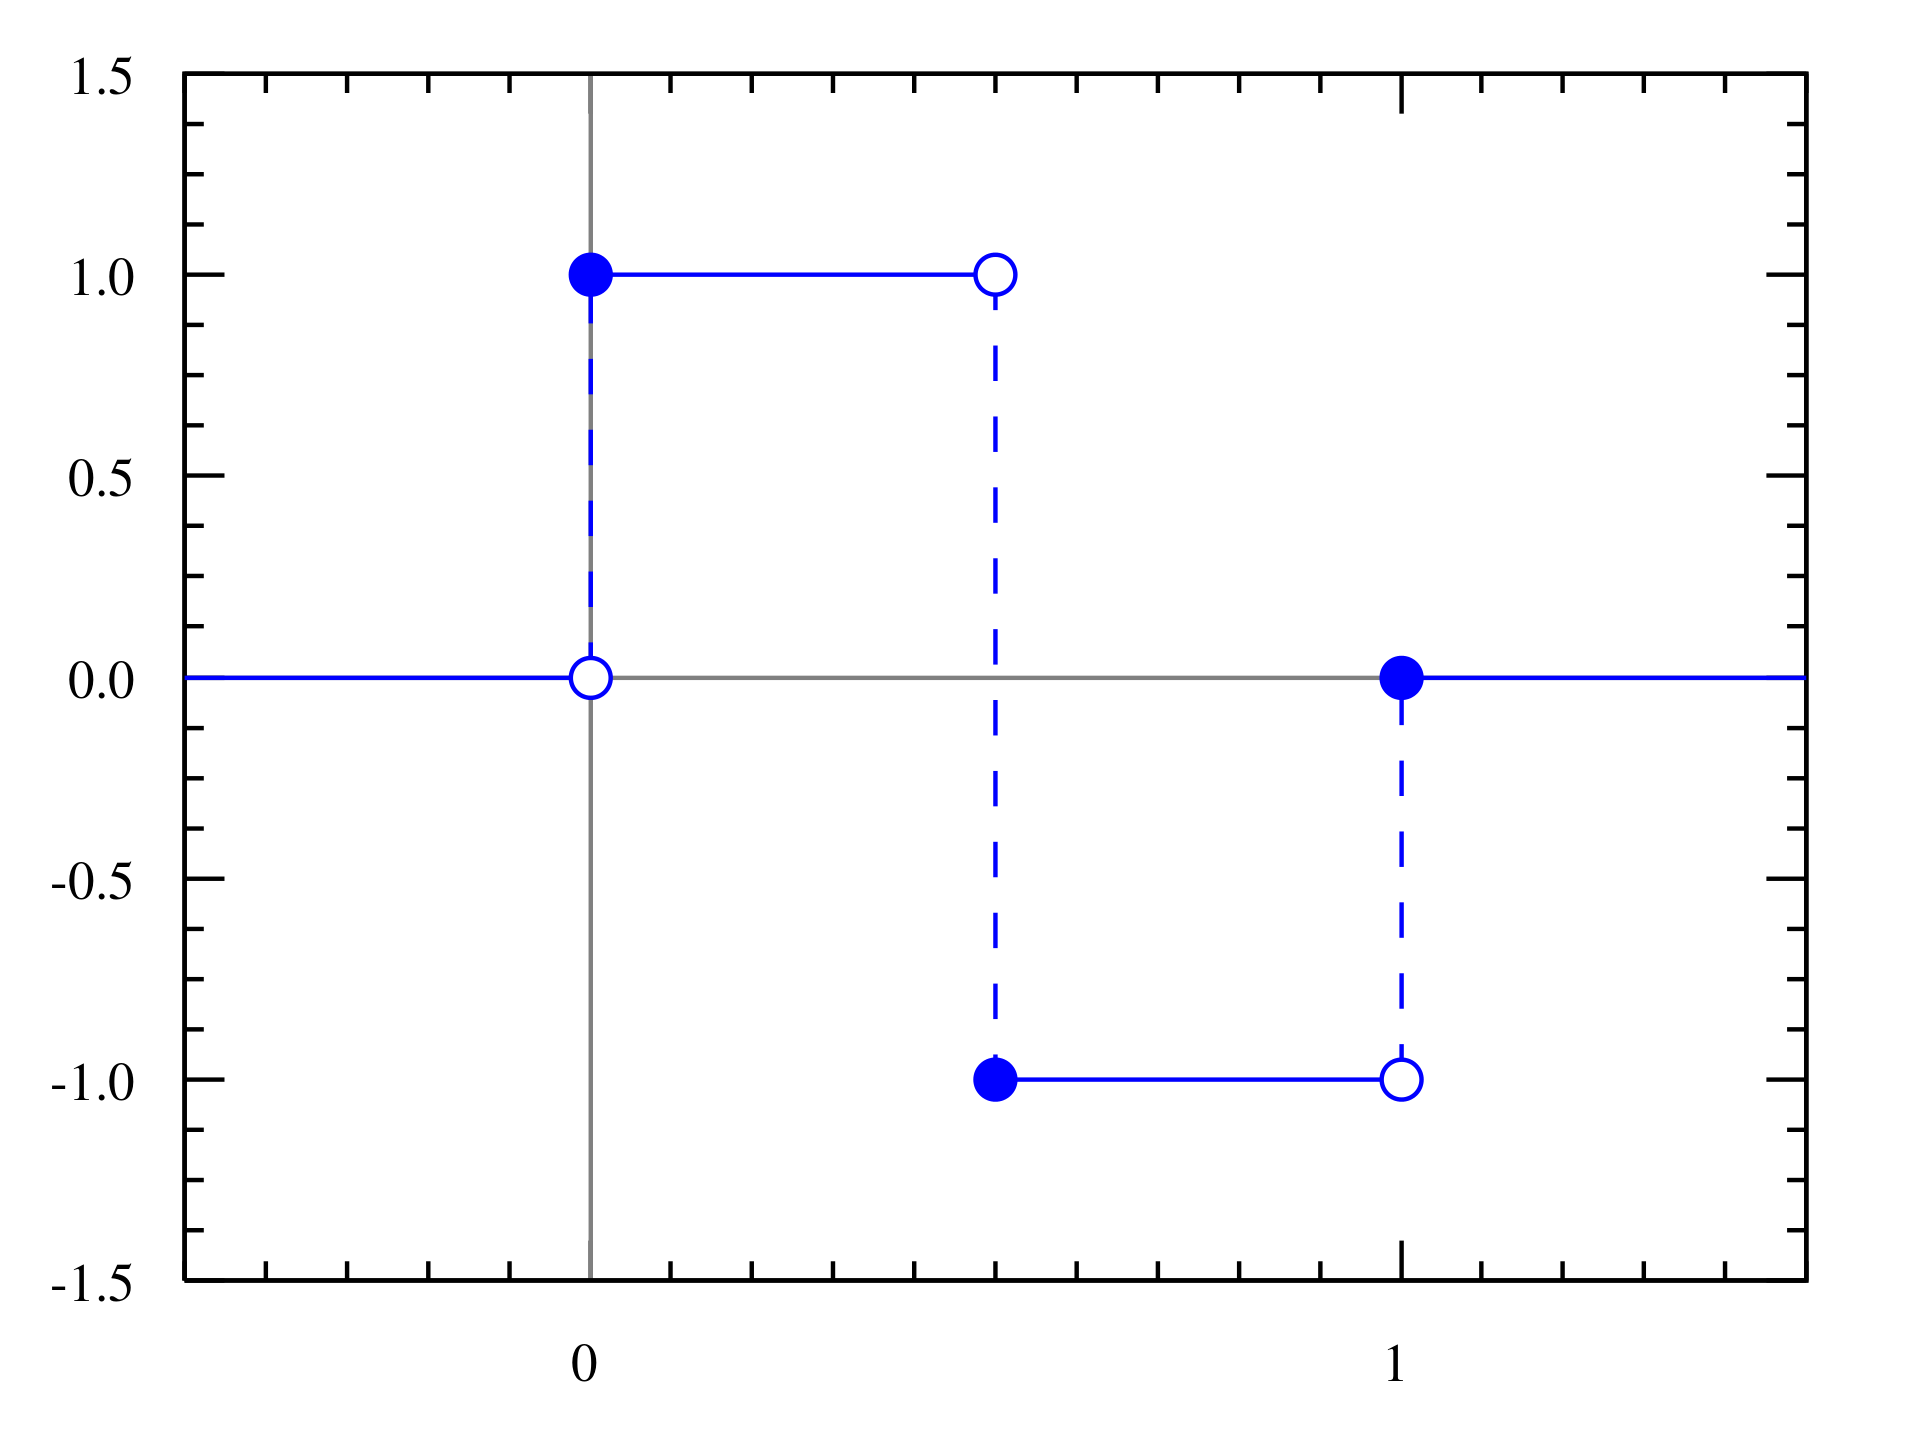
\includegraphics[width=4.5cm]{haar_wavelet.png} & 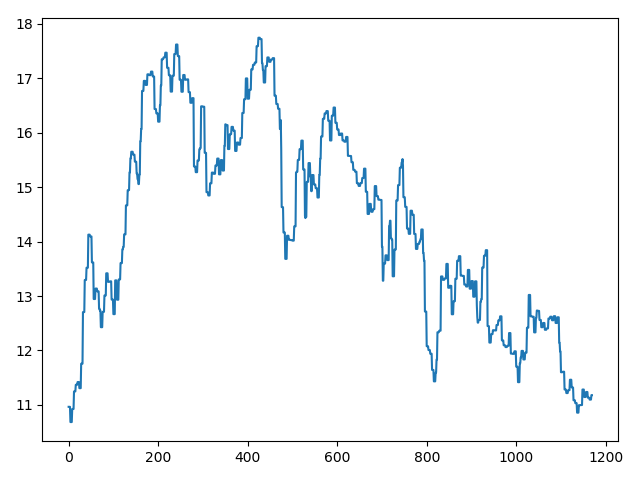
\includegraphics[width=4.5cm]{after_denoising_haar.png} \\
Db4 (Daubechies 4) wavelet \\
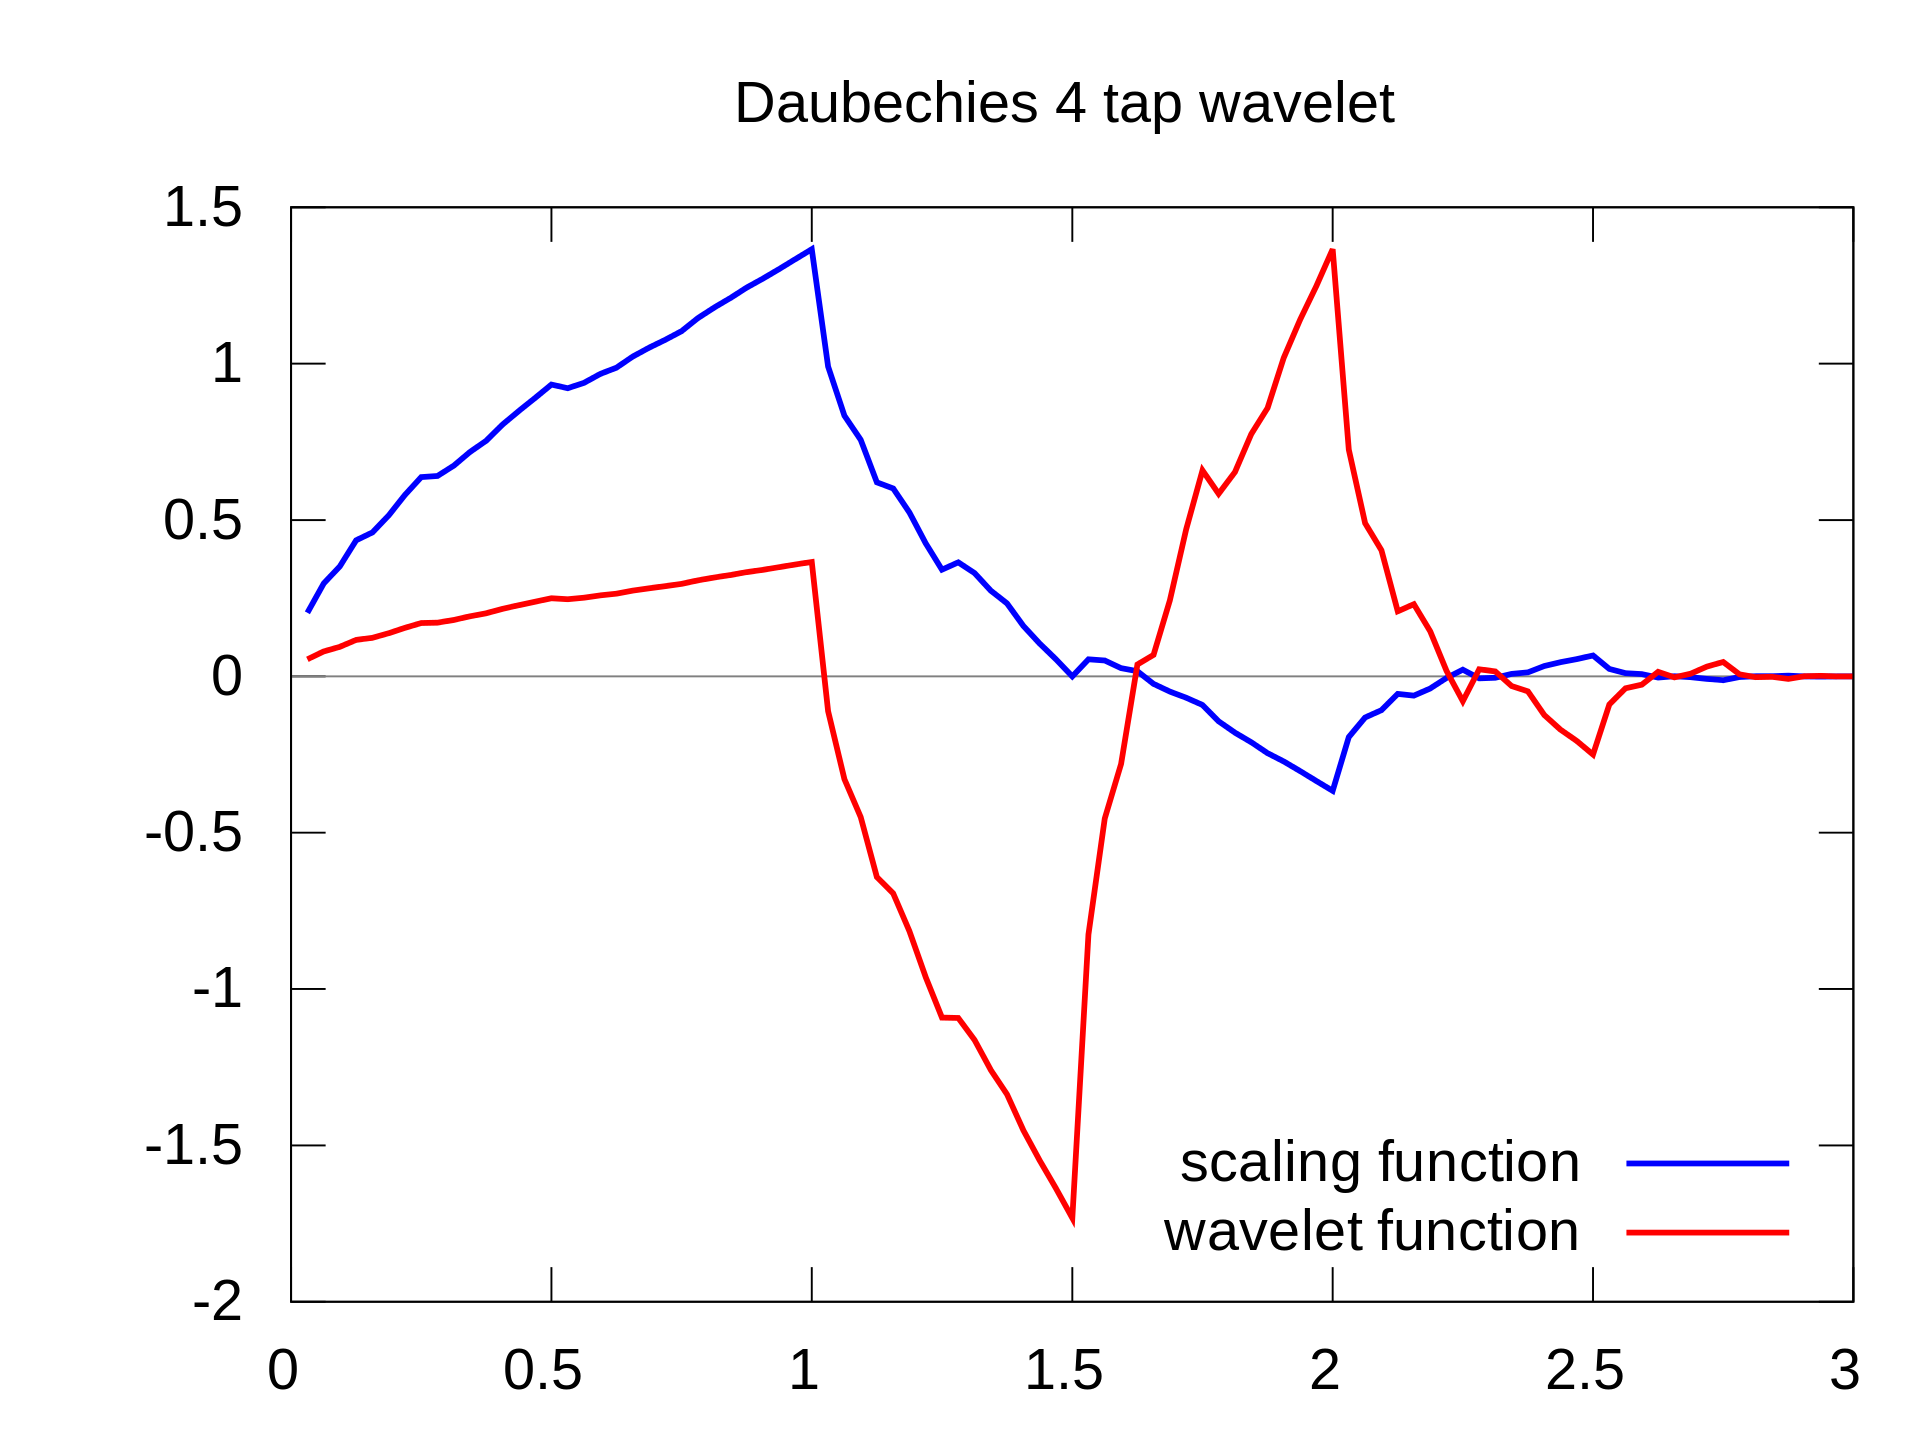
\includegraphics[width=4.5cm]{db4_wavelet.png} & 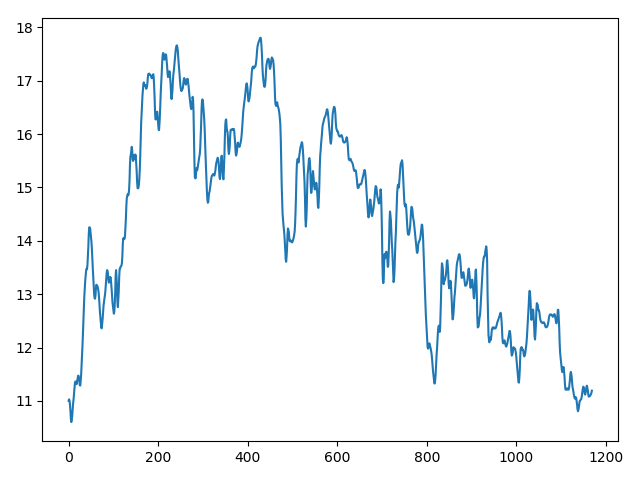
\includegraphics[width=4.5cm]{after_denoising_db4.png} \\
\end{tabular}
\end{center}
\end{frame}

\begin{frame}
\frametitle{AE (Autoencoder)}
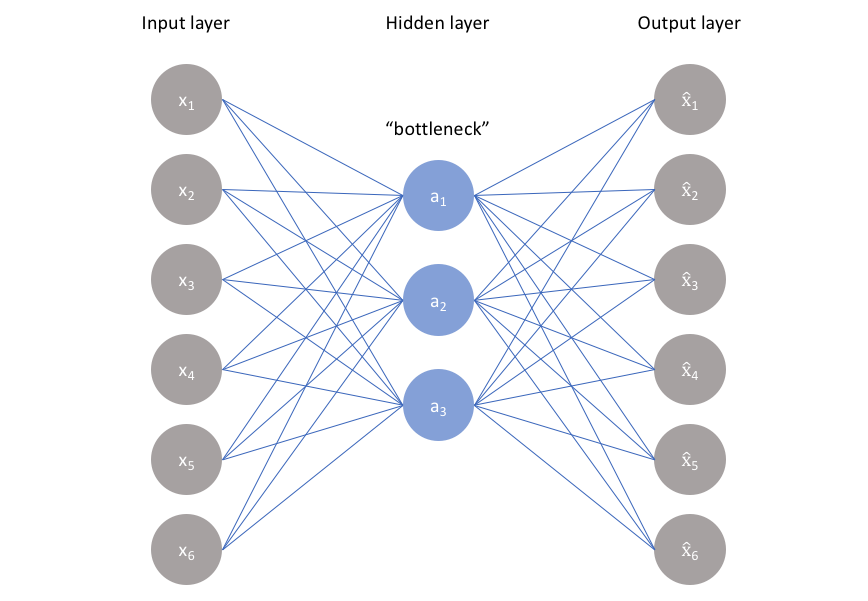
\includegraphics[width=11cm]{sae1.png}
\end{frame}

\begin{frame}
\frametitle{SAE (Stacked Autoencoder)}
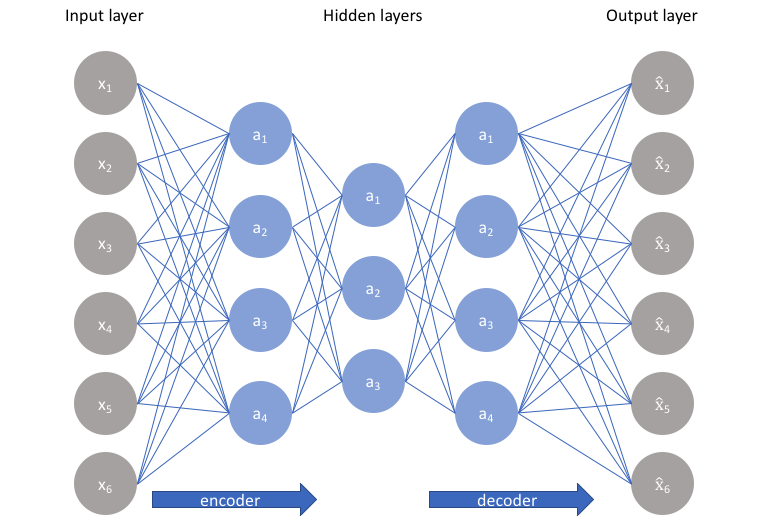
\includegraphics[width=11cm]{sae2.png}
\end{frame}

\begin{frame}
\frametitle{Hidden nodes sensitization}
\begin{minipage}{0.475\textwidth}
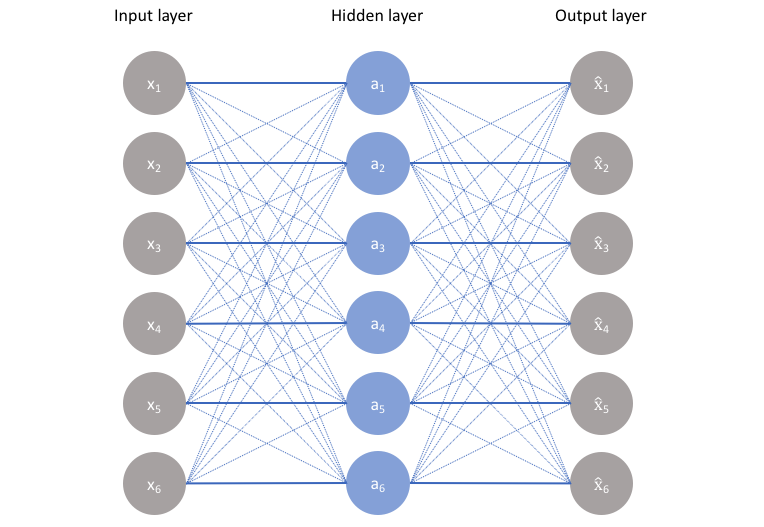
\includegraphics[height=4cm]{sae3.png}
\end{minipage}\hspace{10pt}
\begin{minipage}{0.475\textwidth}
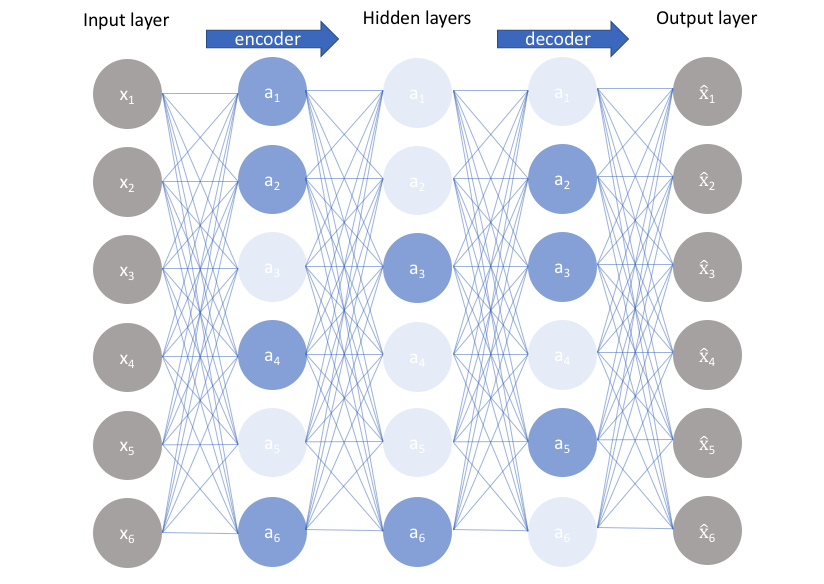
\includegraphics[height=4cm]{sae4.png}
\end{minipage}
\vspace{1cm}
\begin{itemize}
\item When layers sizes are the same, encoders can favorize identity function
\item Neurons activation depens on an input data
\item Kullback-Leibler divergence
\end{itemize}
\end{frame}

\begin{frame}
\frametitle{RNN (Recurrent Neural Network)}
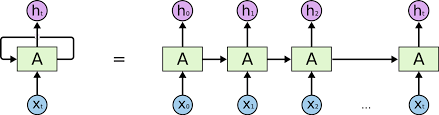
\includegraphics[width=10cm]{rnn.png}\vspace{20pt}
\begin{itemize}
\item $x_i$ -- $i$-th input value 
\item $h_i$ -- $i$-th LSTM output value
\item Learns sequential dependencies
\item Noneffective because of \emph{vanishing gradient problem}
\end{itemize}
\end{frame}

\begin{frame}
\frametitle{LSTM (Long Short Term Memory)}
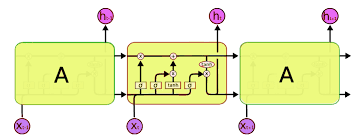
\includegraphics[width=11cm]{lstm.png}
\end{frame}

\begin{frame}
\frametitle{Input data}
\begin{itemize}
\item Base: daily trading data (OHLC + volume) of Ford (* - 30.06.2017)
\item Potentially any additional technical indicators or macroeconomic variables could be used
\end{itemize}
\end{frame}

\begin{frame}
\frametitle{Input data}
\begin{center}
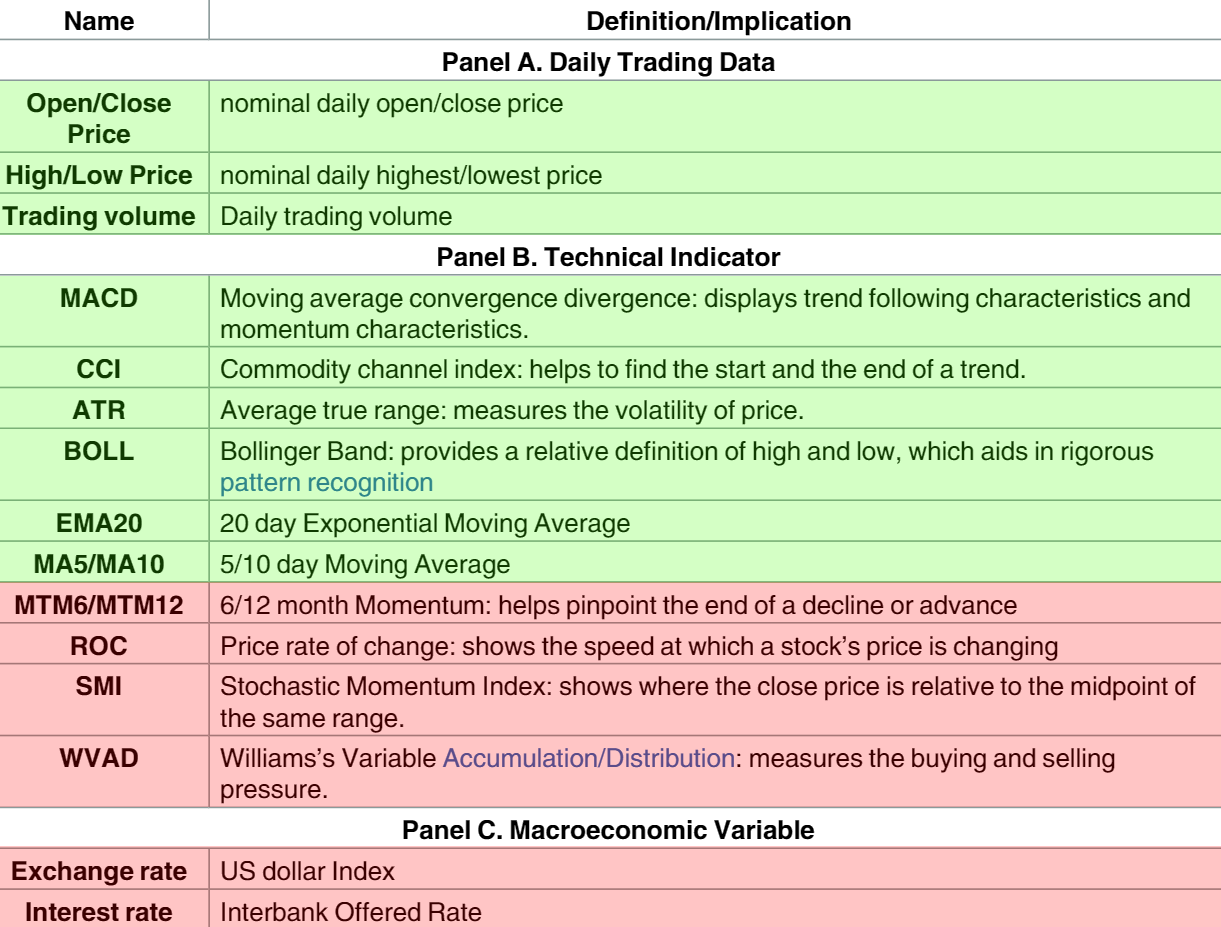
\includegraphics[width=10cm]{summary.png}
\end{center}
\end{frame}

\begin{frame}
\frametitle{Results}

\end{frame}

\end{document}